
\chapter{多渠道广告预算分配算法SVR+Q+MCKP}

在多渠道广告预算分配场景中,营销人员需要将固定预算合理的分配到若干个广告渠道上,以使得在多渠道上产生的长期整体收益最大化。与客户关系管理相同,这也是一个序贯决策问题,因此,非常适合使用强化学习思想进行解决。但是,因为在多渠道广告投放的过程中存在固定预算约束、可获得的数据量少、可变时间间隔等问题,如果直接使用强化学习模型进行求解往往得不到满意的结果。所以,本章首先针对数据量不足、存在固定预算约束的问题,提出了一个基于批学习的SVR+Q+MCKP模型,该模型可以将Q值函数的逼近问题转化为高维空间中线性回归问题,在提高模型的收敛速度的同时对小批量高维度的数据有很好的逼近效果。另外,针对在广告投放过程中存在的可变时间间隔问题,为了使SVR+Q+MCKP模型进行更有效的更新,提出一个归一化因子以及归一化因子的更新方法,用于减少可变时间间隔对奖赏信号带来的噪声影响。

\section{概述}
本节在对多渠道广告预算分配目标进行形式化的描述后,指出考虑使用强化学习思想解决该问题的原因。接着,分析目前强化学习在解决预算分配问题中的相关研究,并在此基础上形成本文的基本思路。最后,针对多渠道广告预算分配场景中存在的特点进行分析,以此作为本章研究的出发点。

\subsection{问题描述}
在本文的第一章中,对基于DSP平台的多渠道广告预算分配场景和机制进行了详细介绍,接下来本小节将结合图$\ref{fig:广告渠道预算分配示意图}$,给出多渠道广告预算分配问题的形式化描述。

考虑在某一次的广告投放过程中,假设给予营销人员在$I$个渠道上投放广告的固定预算金额为$B$,营销人员制定的广告投放的策略为$\bm{x}=(x_{1},x_{2},\cdots,x_{I})$,其中,$x_{i}$表示分配给第$i$个渠道的投放金额,令$R_{all}(\bm{x})$表示为在给定预算分配策略$\bm{x}$下$n$个渠道所能产生的利润之和。可以将营销人员要解决的问题形式化为:
\begin{equation}\label{seq_ad_goal}
\begin{split}
&\max_{\bm{x}} R_{all}(\bm{x}),\\
&s.t. \sum_{i=1}^{I} x_{i} \leqslant B \text{且} x_{i} \geq 0.
\end{split}
\end{equation}

具体来说,营销人员的目标是在给定广告预算$B$下,求得一个可以使的企业获得利润最大化的投放策略$\bm{x}$。但是,在实际应用中,为了能够更好的评价广告渠道的质量,而且为了能达到持久有效的营销效果,营销人员一般都会选择在一个DSP平台下进行为期一年或几年的持续投放。因此,广告投放是一个序贯决策过程,企业追求的是长远收益最大化,即广告所产生的累积收益最大化。所以,如果仅仅考虑即时利润,是不符合企业的最终目标的。

强化学习主要用于序贯决策问题,并以追求累积奖赏最大化为学习目标。所以,如果将广告的即时利润作为奖赏,累积收益作为值函数,那么使用强化学习技术对多渠道广告投放问题进行建模,是最符合业务场景的。

\subsection{研究动机}

% 比如:文献\citep{pednault2002sequential}将与顾客的交互营销行为建模为一个马尔可夫过程,然后提出一种批处理的强化学习算法,进行营销策略的学习。文献\citep{archak2010budget}在MDP框架中提出了一个在线广告资金分配的贪婪算法,文献\citep{boutilier2016budget}通过使用多MDP来代表不同类型的顾客,然后使用线性规划的方法,解决资金的分配问题。但是,
随着强化学习的发展,越来越多的学者和企业开始采用强化学习思想解决营销资金的优化问题,但是,大多数工作都是针对单一市场渠道进行优化的\citep{zhang2017multi},他们的解决方法主要是将客户和渠道的交互数据模拟成一个马尔可夫链,然后使用强化学习求解方法进行策略的学习\citep{,pednault2002sequential,archak2010budget,boutilier2016budget}。但是,这些解决方法都会用到用户的个人信息和交互数据,而在我们的场景中,只有渠道产生的投放效果数据,不存在顾客的数据,因此和我们要研究的多渠道的应用背景不符合。

据调研所知,和本文应用背景相关的文献有两篇,在文献\citep{yang2012budget}中,作者针对多渠道搜索广告竞价问题,首次提出一个分层预算分配框架,包括系统、广告和关键词三层,通过联动机制可以实现这三次预算的自动调整,以最大化长期收益,但是文章只在投放机制和框架的层面进行详细地介绍,并没有对分配策略展开深入的研究。在文献\citep{zhang2017multi}中,作者使用一种启发的二分搜索算法来从投放数据中寻找每个渠道最优的投放花费,并结合MCKP问题,来解决资金的分配问题,但是作者并没有考虑到长期利润最大化的问题。

综合考虑以上相关工作,本文提出一个解决多渠道广告资金分配的研究方案。将文献\citep{pednault2002sequential,archak2010budget,boutilier2016budget}中使用马尔科夫决策过程针对单渠道中的用户建模改为对多渠道本身进行建模,并利用Q-learning算法求出渠道的价值函数,然后通过文献\citep{zhang2017multi}中的MCKP方法来解决最终的资金分配优化问题。但是,这种解决方案仍然面临以下问题:

% 综合考虑以上文献,我们从解决单渠道的资金优化问题出发,将文献\citep{pednault2002sequential}中使用马尔科夫决策过程对用户建模改为对渠道进行建模,然后通过对多渠道广告投放中存在的问题进行分析,进而修改强化学习的奖赏函数来更好的表达渠道的价值函数,最后结合各渠道的价值函数并借助MCKP来解决多渠道的资金分配问题。

首先,对于大部分企业来说,广告投放是以天为单位进行的,所以投放数据量比较少,这会影响模型的训练和学习。另外,因为在广告投放的过程中,因为同一渠道上存在可变时间间隔的问题,会对值函数的学习造成一定的影响;而且,不同渠道间的广告投放效果也会相互影响,如果单单只考虑本渠道投放效果的期望回报,值函数的学习也是不准确的。

本章主要从以上两个方面进行改进。针对第一个问题,利用基于核函数的非参数化函数逼近方法解决小样本下的值函数逼近问题,然后借助文献\citep{pednault2002sequential}中的提出的批学习Q-learning离线学习方法进行学习,最后借助MCKP来解决资金的分配优化问题,形成一个初步的SVR+Q+MCKP算法。
针对第一个问题,从广告渠道的时空影响方面出发,分别提出对应的解决方法,形成最终的SVR+Q+MCKP算法。其中,时间方面,主要考虑单渠道自身的可变长时间间隔问题,空间方面,主要考虑渠道间的广告效果影响问题。

\section{初步SVR+Q+MCKP模型}
\subsection{离线批学习方法}
在Q-learning算法(伪代码:$\ref{algo:algorithm_2}$)这的应用中,存在一个前提假设:agent可以与环境进行在线实时互动,而这在一般的实际应用中很难获得。在文献\citep{pednault2002sequential}中,作者提出了一个批Q-learning学习算法用于离线训练问题,该方法在更新价值函数的时候不再需要真正的采取行为和发生环境状态转移。

作者的主要思路是使用静态数据来表示先前真实的交互纪录。具体来说,训练数据$D$是由状态、行为和奖赏组成的向量$<S_{t},A_{t},R_{t}>_{t=1}^{N}$所构成的,在使用Q-learning进行学习时,首先将原始数据切分为多个情节(episode),每个情节由一系列事件(event)组成,每个事件分别是由状态、行为和奖赏组成的向量,其中,在每个情节中的所有事件都保持了原有的出现顺序,这样在训练的时候,使用当前情节中的行为作为agent所选择的行为,转移到的下一状态就是下一个情节的状态。具体过程参考算法中的第几行。

\subsection{SVR+Q逼近模型}
将强化学习应用在多渠道广告预算分配场景时,其过程可表述为:

交互学习阶段,在某一时刻$t$时,渠道的状态为$S_{t}$,当运营人员采取某个行为(花费金额)$A_{t}$时,渠道会返回一个奖赏信息$R_{t}$(产生的利润),然后渠道就进入了下一个状态$S_{t+1}$,准备下一次的投放。在策略决策时,根据渠道所处的状态,从渠道的值函数中贪婪的选出一个行为,作为最终的投放花费金额。其中,渠道的广告花费看作是强化学习中的行为,而强化学习中的状态可以使用渠道之前的投放纪录进行描述,比如:前$i$日的广告花费、产生的利润等信息。

考虑到该场景的状态空间和行为空间都是大,所以对于值函数的评估要采用函数逼近的方法进行解决。在文献\citep{,pednault2002sequential,archak2010budget,boutilier2016budget}中,针对值函数的逼近学习,作者大多采用参数化线性函数逼近的方法。但是在多渠道广告预算分配场景中,因为可获得的数据量比较少,所以参数化非线性函数逼近的方法常常会因为线性方法表达能力差而很难取得理想的逼近效果。又因为在参数化非线性函数逼近方法中,神经网络的训练也需要大量的训练数据。但是,考虑到基于非参数函数逼近方法的灵活性,并且可以充分利用样本进行训练,所以在本模型中,通过采用基于核函数的支持向量回归(Support Vector Regression, SVR)逼近模型,可以将值函数逼近问题转化为高纬特征空间的线性回归问题,在保证泛化能力的前提先有效提高算法的收敛速度。

为了进一步提高模型的逼近效果,我们采用对每个渠道分别进行函数逼近的方法。另外,对每个渠道$i$的行为空间通过均匀离散化的方法,离散成$M_{i}$个花费行为区间,每个行为值通过该行为区间的花费均值代替,那么最终形成的离散行为可表示为$\{A_{i1},A_{i2},\cdots,A_{iM_{i}}\}$其中$i=1,\cdots,I$,$I$为渠道的个数,

下面介绍SVR-Q值函数逼近模型的构建和逼近过程。

假设当前第$i$个渠道的样本集合为$D_{i}=\{<\bm{X}_{ij}, Q_{ij}>\}_{j=1}^{N_{i}} \subseteq (\bm{S} \times A \times Y)^{N_{i}}$,其中$\bm{X}_{ij}=(\bm{S}_{ij}, A_{ij})$为样本$j$的输入向量,$Q_{ij}$为样本$j$的Q输出值,$N_{i}$为第$i$个渠道的样本数量,$(\bm{S} \times A) = \mathbb{R}^{n+1}$表示输入域,$Y \subseteq \mathbb{R}$表示输出域。

利用SVR-Q对值函数进行逼近时,要以结构化风险最小为目标,学习一组仿射函数$\{f_{i}:(\bm{S} \times A) \mapsto Y\}$,$i=1,\cdots,I$。形式为:
\begin{equation}\label{seq:obj1}
\begin{aligned}
Q_{i}=f_{i}(\bm{s,a})=f_{i}(\bm{x})=\bm{w}_{i}^{T} \bm{\phi}(\bm{x}) + b_{i}, \quad i=1,2,\cdots,I
\end{aligned}
\end{equation}

式\eqref{seq:obj1}中,$\bm{\phi}(\cdot)$表示可以将样本从非线性空间映射到高维线性空间的函数,$\bm{w}$表示线性回归函数的权值向量,$b$是一个偏置项,$Q_{i}$是向量$(\bm{x})$在第$i$个模型的Q输出值。根据SVR的原理,可以将原问题转化为带约束条件的优化问题:

\begin{equation}\label{seq:svr_ori}
\begin{split}
& \min_{\bm{w}_{i}, b_{i},\xi_{i}, \hat{\xi}_{i}}  J(\bm{w}_{i},b_{i},\xi_{i},\hat{\xi}_{i}) = \frac{1}{2} \left \| \bm{w}_{i} \right \|^{2} + C \sum_{j=1}^{N_{i}}(\xi_{ij}+\hat{\xi}_{ij})\\ 
& s.t. \begin{matrix}
& f_{i}(\bm{X}_{ij}) - Q_{ij} \leqslant \epsilon + \xi_{ij}\\
&Q_{ij} - f_{i}(\bm{X}_{ij})  \leqslant \epsilon + \hat{\xi}_{ij} \\
&\xi_{ij} \geqslant 0, \quad \hat{\xi}_{ij} \geqslant 0\\
& i=1,2,\cdots,I \quad j=1,\cdots,N_{i}
\end{matrix}
\end{split}
\end{equation}

式\eqref{seq:svr_ori}中,$\xi_{ij}$,$\hat{\xi}_{ij}$为松弛因子,$C_{i}$是正则化参数,用于控制对超出误差允许范围的样本的惩罚程度,$\bm{w}_{i}$为权值向量,用于控制模型的复杂程度。

引入拉格朗日乘子$\alpha_{ij} \geqslant 0$,$\hat{\alpha_{ij}} \geqslant 0$,$\mu_{ij} \geqslant 0$,$\hat{\mu_{ij}} \geqslant 0$,将原空间的约束优化问题转化为对偶空间的无约束优化问题,得到拉格朗日函数:

\begin{equation}\label{seq_lagrange}
\begin{aligned}
L_{i}(\bm{w}_{i}, b_{i}, \bm{\alpha}_{i}, \bm{\hat{\alpha}}_{i}, \bm{\xi}_{i}, \bm{\hat{\xi}}_{i},
\bm{\mu}_{i},\bm{\hat{\mu}}_{i})&=\frac{1}{2} \left \| \bm{{w}}_{i} \right \|^{2} + C_{i} \sum_{j=1}^{N_{i}}(\xi_{ij} + \hat{\xi}_{ij}) - \sum_{j=1}^{N_{i}}\mu_{ij}\xi_{ij} - \sum_{j=1}^{N_{i}}\hat{\mu}_{ij}\hat{\xi}_{ij} \\ 
&+ \sum_{j=1}^{N_{i}} \alpha_{ij}(\bm{w}^{T} \bm{\phi}(\bm{X}_{ij}) + b_{i} - Q_{ij} - \epsilon - \xi_{ij}) \\
&+ \sum_{j=1}^{N_{i}} \hat{\alpha}_{ij}(Q_{ij} - \bm{w}^{T} \bm{\phi}(\bm{X}_{ij}) - b_{i} - \epsilon - \hat{\xi_{ij}})\\
\end{aligned}
\end{equation}

对式$\eqref{seq_lagrange}$求偏导:
\begin{equation}\label{seq_lag_deri}
\begin{split}
&\frac{\partial{L_{i}}}{\partial{\bm{w}_{i}}}=0 \Rightarrow \bm{w}_{i} = \sum_{j=1}^{N_{i}}(\hat{\alpha}_{ij}-\alpha_{ij})(\bm{X}_{ij})
\\ 
&\frac{\partial{L_{i}}}{\partial{b_{i}}}=0 \Rightarrow 0 = \sum_{j=1}^{N_{i}}(\hat{\alpha}_{ij}-\alpha_{ij})
\\ 
&\frac{\partial{L_{i}}}{\partial{\xi_{ij}}}=0 \Rightarrow  C_{i} = \alpha_{ij} + \mu_{ij}
\\ 
&\frac{\partial{L_{i}}}{\partial{\hat{\xi}_{ij}}}=0 \Rightarrow  C_{i} = \hat{\alpha_{ij}} + \hat{\mu_{ij}}
\\
\end{split}
\end{equation}

将式\eqref{seq_lag_deri}求导结果代入式\eqref{seq_lagrange},即可得到SVR的对偶问题:

\begin{equation}\label{seq_lagr_dual}
\begin{split}
&\max_{\bm{\alpha}_{i}, \bm{\hat{\alpha}}_{i}} \sum_{j=1}^{N_{i}} Q_{ij}(\hat{\alpha}_{ij} - \alpha_{ij}) - \epsilon (\hat{\alpha}_{ij} + \alpha_{ij}) - \frac{1}{2} \sum_{j=1}^{N_{i}} \sum_{k=1}^{N_{i}}(\hat{\alpha_{ij}}-\alpha_{ij})(\hat{\alpha}_{ij}-\alpha_{ij})\bm{X}_{ij}^{T}\bm{X}_{ij},\\
&s.t. \sum_{j=1}^{N_{i}}(\hat{\alpha}_{ij}-\alpha_{ij})=0, \quad 0 \leqslant \alpha_{ij},\hat{\alpha}_{ij} \leqslant C.
\end{split}
\end{equation}

上述过程满足KKT(Karush-Kuhn-Tucker)最优化条件,即需要:
\begin{equation}
\label{seq_kkt}
\left\{\begin{matrix}
&\alpha_{ij}(\bm{w}_{i}^{T} \bm{\phi}(\bm{X}_{ij}) + b_{i} - Q_{ij} - \epsilon - \xi_{ij})=0
\\ 
&\hat{\alpha}_{ij}(Q_{i} - \bm{w}_{i}^{T} \bm{\phi}(\bm{X}_{ij}) - b_{i} - \epsilon - \hat{\xi}_{ij})=0
\\ 
&\alpha_{ij}\hat{\alpha}_{ij}=0, \xi_{ij}\hat{\xi}_{ij}=0
\\ 
&(C_{i}-\alpha_{ij})\xi_{ij}=0,\quad (C_{i}-\hat{\alpha}_{ij})\hat{\xi_{ij}}=0,
\\
\end{matrix}\right.
\end{equation}

将上述结果,可得SVR的解为:
\begin{equation}
\label{seq_svr_final}
f_{i}(\bm{x})=\sum_{j=1}^{N_{i}}(\hat{\alpha}_{ij}-\alpha_{ij})\bm{X}_{ij}^{T}\bm{X}+b_{i}
\end{equation}

在求解$\bm{X}_{ij}^{T}\bm{X}$这个内积的时候,如果输入样本线性不可分,我们可以通过$\bm{\phi}(\cdot):X \to F$函数映射,将输入样本映射到另外一个高维空间并使其线性可分。通常会选择满足Mercer定理的核函数$\bm{k}(\cdot,\cdot)$。目前应用较多的核函数有线性核函数、多项式核函数、RBF以及Sigmoid核函数等,考虑到RBF核函数简单性、计算难度小、算法易于实现等优点,故在本模型中采用RBF核函数,将优化问题表示为关于核函数的线性问题。
\begin{equation}
\bm{k}(\bm{x}_{a} - \bm{x}_{b}) = \exp{\frac{-\left \| \bm{x}_{a} - \bm{x}_{b} \right \|^{2}}{2\sigma^{2}}}
\end{equation}

所以,式$\eqref{seq_svr_final}$可化为:
\begin{equation}\label{seq_final}
\text{Q}_{i}=f_{i}(\bm{x})=f_{i}(\bm{s},a)=\bm{w}_{i}^{T} \bm{\phi}(s,a) + b_{i}=\sum_{j=1}^{N_{i}}(\hat{\alpha}_{ij}-\alpha_{ij})\bm{k}((\bm{s},a),(\bm{S}_{ij},A_{ij}))+b_{i}
\end{equation}
% 式$\eqref{seq_final}$中的b是式$\eqref{seq_kkt}$
以上就是利用SVR+Q模型对第$i$个渠道的值函数进行逼近的方法。

\subsection{MCKP预算分配优化问题}
在使用SVR+Q模型求解完每个渠道的值函数$\text{Q_{i}}$后,我们面临的问题是:对于处于状态$S_{it}$的每个渠道$i$,如何在固定预算$B$下,从各自的行为空间$\{A_{i1},A_{i2},\cdots,A_{iM_{i}}\}$中选择最佳的行为,以使的累积的期望奖赏最大化。如果将$n$个渠道对应$n$类物品,第$i$个渠道中的$M_{i}$个离散花费行为对应第$i$类中的$M_{i}$个不同的物品,给定的固定预算$B$对应背包的总重量$W$。那么,最终的预算分配问题就可以形式化为一个多选择背包问题:

% 通过SVR+Q多路逼近模型进行建模求解后,目前,我们可以得到如下信息:共存在$n$个渠道,并且在每个渠道$i$下,离散后的花费行为空间为:$A_{i}=\{a_{i1},a_{i2},\cdots,a_{i n_{i}}\}$,其中,$n_{i}$为第$i$个花费行为空间的离散行为个数,并且得到了该渠道下的估计值函数:$Q_{i}(\bm{s}_{i},a_{i})$,我们的目标是在给定总预算$B$下,从每个渠道中选择合适的花费行为,使的可以可获得整体价值最大化。巧合的是,该问题可以形式化为一个多选择背包问题。
\begin{equation}\label{seq_mckp}
\begin{split}
&\max \sum_{i=1}^{I}\sum_{j=1}^{N_{i}}\text{Q}_{i}(\bm{S}_{ij}, A_{ij})y_{ij},\\
&s.t. \sum_{i=1}^{I}\sum_{j=1}^{N_{i}}A_{ij}y_{ij} \leqslant B,\\
&\sum_{j=1}^{N_{i}}y_{ij}=1, (i=1,2,\cdots,I),\\
&\forall i,j, \quad y_{ij}=\{0,1\}.\\
\end{split}
\end{equation}

式\eqref{seq_mckp}中,$Q_{ij}(\bm{S}_{ij}, A_{ij})$表示在状态$\bm{S}_{ij}$下第$i$个渠道中第$j$个花费行为所对应的Q值,$A_{ij}$表示第$i$个渠道的第$j$个离散化后的花费行为,$y_{ij}$表示第$i$个渠道中第$j$个花费行为是否被选中,是则取值为1,否则为0。$\sum_{j=1}^{n_{i}}y_{ij}=1$表示$n$个等式约束,意味着每个渠道必须而且只能选择一个花费行为。

% 多选择背包问题具体描述如下:要选进背包的物品被分为互相排斥的$n$类,设第$i$类中有个$n_{i}$不同的物品。从每类中选择且必须选择一个物品放进背包,使得在物品总重量不超过背包承重$W$的前提下,总费用最小化(或总价值最大化)。其模型是一个01整数线性规划问题。
\subsection{批学习SVR-Q-MCKP框架}
综合上述批学习思想、SVR-Q逼近模型以及MCKP算法,就可以得到基于批学习的SVR-Q-MCKP的算法框架,其伪代码如算法$\ref{algo:RBF-SVR+Q}$所示。

在伪代码$\ref{algo:RBF-SVR+Q}$中,训练数据$D$由$n$个渠道的样本集合$D_{i}$组成,每个渠道$i$的样本集合$D_{i}$含有$l_{i,j}$个情节组成,每个情节由一系列事件组成,每个事件包含状态、行为和奖赏信息。在情节数据中,保持了事件原有的出现顺序,以此来重现交互的过程。在第一次迭代中,基于事件中的输入状态和输入行为使用SVR-Q模型来预测即刻奖赏函数,将其作为初步的估计值函数。在随后的迭代中,再使用Q迭代公式更新每个状态行为值,然后再次使用SVR-Q模型逼近Q值函数。按照这种方法逼近所有渠道的Q值函数,最后使用MCKP算法再预算$B$下输出最终的投放策略。另外,对算法中学习了$\alpha_{i}$的选取,设置为$\alpha_{i}=\frac{1}{K}$,目的是让学习的步伐随着迭代次数的增加不断减小。

\begin{algorithm}[htbp]
\small
\SetAlgoLined
\SetKwRepeat{Repeat}{repeat}{until} 
\KwData{预算金额$B$,折扣因子$\gamma_{i}$,正则化参数$C_{i}$,RBF核函数的宽度$\sigma_{i}$,最大迭代次数$P_{i}$,原始样本$D=\{D_{i}|i=1,\cdots,I\}$,其中$D_{i}=\{e_{i,j}|j=1,\cdots,h_{i}\}$,$e_{i,j}=\{<S_{i,j,k}, A_{i,j,k}, R_{i,j,k}>|k=1,\cdots,l_{i,j}\}$,($D_{i}$表示第$i$个渠道的样本,$e_{i,j}$表示第$i$个渠道第$j$个情节,$l_{i,j}$为$e_{i,j}$的长度)}

\KwResult{输出预算分配策略,$\Pi$}

\For{$i = 1$ \KwTo $I$}{
	\For{all $e_{i,j} \in D_{i}$}{
		初始化第$i$个渠道第$j$个情节的的数据:$D_{i,j}^{(0)}=\{<S_{i,j,k}, A_{i,j,k}, R_{i,j,k}>|k=1,\cdots,l_{i,j}\}$\;
	}
	整合第$i$个渠道的全部数据,$D_{i}^{(0)}=\cup_{j=1,\cdots,h_{i}} D_{i,j}^{(0)}$\;
	利用样本$D^{(0)}$,使用公式$\eqref{seq_final}$逼近值函数$Q_{i}^{(0)}$\;
	\For{$p=1$ \KwTo $P$}{
		\For{all $e_{i,j} \in D_{i}$}{
			\For{$k$ \KwTo $l_{i,j}-1$}{
				$v_{i,j,k}^{(p)}=Q^{(p-1)}(S_{i,j,k},A_{i,j,k}) + \alpha_{i} (R_{i,j,k} + \gamma_{i} \max_{a} Q^{(p-1)}(S_{i,j,k+1},a)-Q^{(p-1)}(S_{i,j,k},A_{i,j,k}))$\;
				更新第$j$个情节的样本:$D_{i,j}^{(p)}=\{<S_{i,j,k}, A_{i,j,k}, v_{i,j,k}^{(p)}>|k=1,\cdots,l_{i,j}-1\}$\;
			}
		}
		整合第$i$个渠道的样本:$D^{(p)}_{i}=\cup_{j=1,\cdots,h_{i}}D_{i,j}^{(p)}$\;
		利用样本$D^{(p)}_{i}$,使用公式$\eqref{seq_final}$逼近值函数$Q_{i}^{(p)}$\;
	}
	输出最终的逼近值函数$Q_{i}^{(P)}$\;
}
整合所有渠道的值函数:$Q=\cup_{i=1,\cdots,I} Q_{i}$\;
利用MCKP算法求出分配策略:$\Pi=\text{MCKP}(B,Q)$\;
\caption{SVR-Q-MCKP算法}
\label{algo:RBF-SVR+Q}
\end{algorithm}


\section{基于可变时间间隔SVR+Q+MCKP算法}
本节以两个渠道为例,考察广告在多渠道投放过程的相互影响,如
图$\ref{fig:2_ad_process}$所示为广告在渠道$i$和渠道$j$上投放时的生命周期过程。

% 假设我们于$t_{k}$时刻在渠道$i$上投放一条广告(此广告可以用$A_{ik}$表示),我们可以清楚的发现,广告$A_{ik}$不仅对渠道$i$上$k$时刻以后的广告产生影响,而且还会对渠道$j$上$k$时刻以后的的广告效果产生影响。前者记为渠道的延迟影响,后者记为渠道间的影响。所以,我们在估计广告$A_{ik}$的真实价值时,应该将这两方面都考虑进去。

另外,在广告投放的过程中,同一渠道上广告投放的决策点之间存在可变时间间隔的问题。比如,在渠道$i$上,不是每一天都会进行广告投放,相邻的两个投放时间之间是有一定的时间间隔的,而且这种间隔不是固定的。但是,在标准马尔科夫决策过程中,存在的假设提前是,每两个决策点之间的时间间隔是固定不变的,所以如果按照\eqref{seq:reward}的方式计算累积奖赏,会带来一定的噪声影响。

\begin{figure}[htbp]
\centering
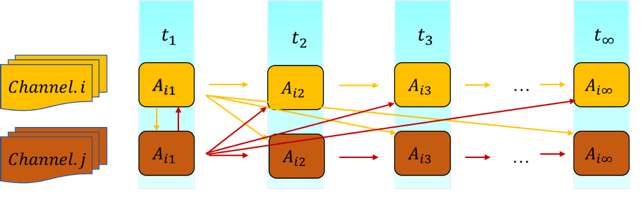
\includegraphics[width=0.8\textwidth]{2_ad_process}
\caption{广告在两个渠道上的生命周期}
\label{fig:2_ad_process}
\end{figure}

和标准的马尔科夫决策过程相比,在带有可变时间间隔的马尔科夫决策过程中,每次的交互事件都会被标记上时间。假设将初始状态的时刻记为0,那么后续交互事件被标记的时间都大于0。比如,整个马尔科夫决策过程是从$t_{1}=0$时刻开始的,并且初始状态为$S_{1}$,之后agent重复的采取行为,便会得到一系列的由行为、状态、奖赏以及时间组成的四元组$\{<S_{i},A_{i},R_{i},t_{i}>\}_{i=1}^{\infty}$。那么在计算累积折扣奖赏时,折扣因子就被定义为关于时间的函数,如式\eqref{seq:r}所示:
\begin{equation}\label{seq:r}
\begin{aligned}
G_{t}=\sum_{i=1}^{\infty} \gamma^{t_{i}}R_{i}
\end{aligned}
\end{equation}

在可变时间间隔的马尔科夫决策过程中,需要为可变长时间间隔中的奖赏找到一个合适的归一化方法,以减少可变时间间隔给奖赏的计算所带来的噪声。那么,为了估计即时奖赏,普遍采用的方法是将时间间隔内的奖赏除以时间间隔的方式来进行归一化。但是在更新Q值函数的时候会变的很复杂。因为在Q函数的更新过过程中,时间间隔也会受到学习率的影响,所以,如果只进行期望累积奖赏的更新而不尽兴时间间隔的更新,那么就会在更新的过程中产生偏差。所以,为了解决这个问题,本节提出了一个归一化因子,用于计算归一化时的有效时间间隔,具体来说,就是按照Q函数的更新方法来更新归一化因子,以使的Q值和时间间隔保持同步更新。结合以上的想法,本节提出了一个针对可变时间间隔的SVR-Q-MCKP学习方法如$\ref{algo:RBF-SVR-Q-t}$所示,其中,第19行为Q值$v_{i,j,k}^{(p)}$的更新方法,第20行为归一化因子$Z^{(p)}_{i,j,k}$的更新方法。
\begin{algorithm}[htbp]
\small
\SetAlgoLined
\SetKwRepeat{Repeat}{repeat}{until} 
\KwData{预算金额$B$,折扣因子$\gamma_{i}$,正则化参数$C_{i}$,RBF核函数的宽度$\sigma_{i}$,最大迭代次数$P_{i}$,原始样本$D=\{D_{i}|i=1,\cdots,I\}$,其中$D_{i}=\{e_{i,j}|j=1,\cdots,h_{i}\}$,$e_{i,j}=\{<S_{i,j,k}, A_{i,j,k}, R_{i,j,k}, t_{i,j,k}>|k=1,\cdots,l_{i,j}\}$,($D_{i}$表示第$i$个渠道的样本,$e_{i,j}$表示第$i$个渠道第$j$个情节,$l_{i,j}$为$e_{i,j}$的长度)}

\KwResult{输出预算分配策略,$\Pi$}

\For{$i = 1$ \KwTo $I$}{
	\For{all $e_{i,j} \in D_{i}$}{
		\For{$k$ \KwTo $l_{i,j}$}{
			计算时间间隔,$\triangle t_{i,j,k}=t_{i,j,k+1}-t_{i,j,k}$\;
		}
	}
	\For{all $e_{i,j} \in D_{i}$}{
		\For{$k$ \KwTo $l_{i,j}-1$}{
			得到初始的归一化因子:$Z^{(0)}_{i,j,k}=\triangle t_{i,j,k}$\;
			得到初始的奖赏值:$v^{(0)}_{i,j,k} = R_{i,j,k}$\;
			将奖赏值进行归一化:$D_{i,j}^{(0)}=\{<S_{i,j,k}, A_{i,j,k}, \frac{v^{(0)}_{i,j,k}}{Z^{(0)}_{i,j,k}}>|k=1,\cdots,l_{i,j}\}$\;
		}
	}
	整合第$i$个渠道的全部数据,$D_{i}^{(0)}=\cup_{j=1,\cdots,h_{i}} D_{i,j}^{(0)}$\;
	使用公式$\eqref{seq_final}$逼近值函数$Q_{i}^{(0)}$\;
	\For{$p=1$ \KwTo $P$}{
		\For{all $e_{i,j} \in D_{i}$}{
			\For{$k$ \KwTo $l_{i,j}-1$}{
				$v_{i,j,k}^{(p)}=(1-\alpha_{i})Q^{(p-1)}(S_{i,j,k},A_{i,j,k}) \cdot Z^{(p-1)}_{i,j,k} + \alpha_{i} (R_{i,j,k} + \gamma_{i}^{\triangle t_{i,j,k}} \max_{a} Q^{(p-1)}(S_{i,j,k+1},a) \cdot Z^{(p-1)}_{i,j+1,k})$\;
				$Z^{(p)}_{i,j,k}=(1-\alpha_{i})Z^{(p-1)}_{i,j,k}+\alpha_{i}(\triangle t_{i,j,k} + \gamma_{i}^{\triangle t_{i,j,k}} \cdot Z^{(p-1)}_{i,j+1,k})$\;
				更新第$j$个情节的样本:$D_{i,j}^{(p)}=\{<S_{i,j,k}, A_{i,j,k}, \frac{v_{i,j,k}^{(p)}}{Z^{(p)_{i,j,k}}}>|k=1,\cdots,l_{i,j}-1\}$\;
			}
		}
		整合第$i$个渠道的样本:$D^{(p)}_{i}=\cup_{j=1,\cdots,h_{i}}D_{i,j}^{(p)}$\;
		利用样本$D_{i}^{(p)}$,使用公式$\eqref{seq_final}$逼近值函数$Q_{i}^{(p)}$\;
	}
	输出最终的逼近值函数$Q_{i}^{(P)} = Q_{i}^{(P)} \cdot Z^{(P)}_{i}$\;
}
整合所有渠道的值函数:$Q=\cup_{i=1,\cdots,I} Q_{i}$\;
利用MCKP算法求出分配策略:$\Pi=\text{MCKP}(B,Q)$\;
\caption{基于可变时间间隔的SVR-Q-MCKP算法}
\label{algo:RBF-SVR-Q-t}
\end{algorithm}


% 一个自然的想法是可以使用均值奖赏的方式进行归一化,即在$\triangle t_{i}=t_{i+1}-t_{i}$间隔内的归一化奖赏等于该间隔内的得到的奖赏$R_{i}$除以该时间间隔$\triangle t_{i}$,即 $R_{i}=\frac{R_{i}}{\triangle t_{i}}$。在得到归一化的即刻奖赏后,算法$\ref{algo:RBF-SVR+Q}$中第10行的Q值函数的更新公式就变为了:
% \begin{equation}\label{seq:q_inter}
% \begin{aligned}
% v_{i}=(1-\alpha) Q(S_{i},A_{i}) \cdot \triangle t_{i} + \alpha (R_{i} + \gamma^{\triangle t_{i}} \max_{a} Q(S_{i},a) \cdot \triangle t_{i})\;
% \end{aligned}
% \end{equation}

% 从公式\eqref{seq:q_inter}可以看出,因为$R_{i}$的计算使用了时间间隔$\triangle t_{i}$,所以在每次的迭代过程中,时间间隔$\triangle t_{i}$会受到学习率的影响。也就是说,我们在使用公式\eqref{seq:q_inter}更新v_{i}值的时候



% 但是在进行均值归一化时,如果仍然除以$\triangle t_{i}$会带来以下的后果:随着迭代次数的增加,因为奖赏值$v_{i}$在不断的改变,而如果$\triangle t_{i}$的方式进行更新,那么必然会带来偏差,因为此时$v_{i}$在不断变化,而$\triangle t_{i}$是不变的。因为这个问题,我们要对时间间隔$\triangle t_{i}$进行不断的更新,依照Q函数的更新方法,本文提出一个针对时间间隔的更新方法(下式\eqref{seq:q_inter_t}),用于解决时间间隔可变的Q-learning学习问题,记初始时归一化因子$Z_{i}=\triangle t_{i}$:
% \begin{equation}\label{seq:q_inter_t}
% \begin{aligned}
% Z_{i}=(1-\alpha) \cdot Z_{i} + \alpha (\triangle t_{i} + \lambda^{\triangle t_{i}}  \cdot Z_{i})\;
% \end{aligned}
% \end{equation}


% \subsection{渠道之间的影响}
% 如本节开头所述,某一时刻在某一渠道上投放的广告不仅会在该渠道的后续时间里产生影响(延迟奖赏),而且还会对其他渠道产生影响(渠道间影响)。那么,在评价渠道广告的期望价值时,应该将该广告对其他渠道产生的价值考虑进去。

% 这部分因素考虑进去。而在评价对其他渠道产生的影响时,本节假设一个渠道$i$对另一个渠道$j$的影响程度和他们的花费资金是正相关的,而这个假设也是符合广告投放的业务场景的。所以:

% 假设含有$I$个渠道的集合为$C=\{1,2,\cdots,I\}$,在某时刻,渠道$i$对其他渠道$C\backslash\{i\}$产生的期望奖赏可以记为$q_{i}^{'}$:

% \begin{equation}\label{seq_ad_influence}
% \begin{aligned}
% q_{i}^{'}=\sum_{j\in C \backslash \{i\}} \sum_{k=0}^{\infty} \tau_{j,i,t+k+1} \cdot \gamma_{i}^{k} \cdot r_{j,t+k+1}, \quad
% \tau_{j,i,t+k+1}=d \cdot \frac{c_{j,t+k+1}}{c_{i,t+k+1}},d<1.
% \end{aligned}
% \end{equation}

% 式$\eqref{seq_ad_influence}$中,$\gamma_{i}$表示渠道$i$的折扣因子,$\tau_{j,i,t+k+1}$是一个常数$d$乘以$t+k+1$时刻在第$j$个渠道上的花费与在第$i$个渠道上花费之比,$r_{j,t+k+1}$表示渠道$j$在$t+k+1$时刻所获的即时利润。从公式中可以看出,$\sum_{k=0}^{\infty} \gamma_{i}^{k} \cdot r_{j,t+k+1}$是近似为其他某一渠道获得的所获的累积利润,$\tau_{j,i,t+k+1}$通过某时刻第$j$个渠道上的花费与第$i$个渠道上花费的比值来反映渠道$j$对渠道$i$的投放效果的影响。

% 于是,考虑$q_{i}^{'}$并结合公式\eqref{seq2_qsa},可以得到改进的渠道$i$最优值函数的公式:
% \begin{equation}
% \label{seq_modified_q}
% \begin{aligned}
% q_{i}(S_{t},A_{t})&=\mathbb{E}[\sum_{k=0}^{\infty} \gamma_{i}^{k} r_{i,r+k+1} + \sum_{j \in I \backslash \{i\}} \sum_{k=0}^{\infty} \tau_{j,i,t+k+1} \cdot \gamma_{i}^{k} r_{j,t+k+1} | S_{t}=s, A_t = a]\\
% &=\mathbb{E}[r_{i,t+1} + \gamma_{i} \sum_{k=0}^{\infty} \gamma_{i}^{k} r_{r+k+2} + \sum_{j \in \backslash \{i\}} \tau_{j,i,t+1}r_{j, t+1} \\
% &+ \gamma_{i} \sum_{j \in \backslash \{i\}} \sum_{k=0}^{\infty} \tau_{j,i,t+k+2} \cdot \gamma_{i}^{k} r_{j,t+k+2} | S_{t}=s, A_t = a]\\
% &=\mathbb{E}[r_{i,t+1} + \sum_{j \in I \backslash \{i\}} \tau_{j,i,t+1} r_{j, t+1} + \gamma_{i} q_{i}(S_{t+1},A_{t+1}) | S_{t}=s, A_t = a]\\
% \end{aligned}
% \end{equation}

% 因此,我们就可以将$t$时刻渠道$i$的Q值迭代的更新公式改为:
% % \begin{equation}
% % \begin{aligned}
% \begin{dmath}
% \label{seq_modified_Q}
% Q_{i}(S_{t},A_{t})=Q_{i}(S_{t},A_{t})+\alpha_{i}(r_{i, t+1} + \sum_{j \in I \backslash \{i\}} \tau_{j,i,t+1} r_{j, t+1} + \gamma_{i} max_{a_{'}} Q_{i}(S_{t+1}, a^{'}) - Q_{i}(S_{t},A_{t}))
% % \end{aligned}
% % \end{equation}
% \end{dmath}


% 这一节,首先介绍了在直复营销体系下,基于第三方广告代理商进行广告投放的应用场景及其具体的投放过程。然后,说明了多渠道广告投放的目标是追求全渠道的LTV最大化,以此作为选择强化学习解决该问题的依据。最后,介绍了在广告投放预算分配场景中所面临的三个特点,并针对这些特点进行分析,提出对应的解决思路,来作为本章研究的出发点。

% \subsection{广告预算分配场景}
% 美国直复营销协会(American Direct Marketing Association,ADMA)\footnote{http://www.the-dma.org/}将直复营销(Direct Response Marketing)定义为一种市场营销体系,运用一种或几种广告媒介在任何地点产生可以度量的反应或交易。直效营销仅仅属于直复营销中的一种应用场景,它特指不通过第三方,中间人,而直接对客户进行推广和营销,以维持企业与客户的良好关系。但是,在此场景下需要企业有充足的客户资源和大量的相关客户资料,这对于大部分企业是很难办到的,因为它需要很长时间的积累,特别是在日益激烈的市场竞争环境中,时间就是企业的生命。于是,为了快速获取用户、推广相关产品、扩大公司的收入,越来越多的企业选择通过第三方广告代理商(ad-agency)进行广告投放。

% 广告代理商除了帮助企业进行广告设计与策划以外,还有一部分更重要的工作,就是帮助广告主安排或代为购买媒介空间或时间。近年来,随着广告市场的不断发展和扩大,为了方便广告主高效的进行广告投放,大部分在线的广告代理商都建设了自己的广告投放平台,其投放流程如图

% $\ref{fig:ad_process}$
% 所示:在广告投放平台上,广告代理商(ad-agency)有很多可供选择的广告渠道(channel)资源,广告主在每次进行广告投放时需要提供一个广告投放策略,策略的内容包括在哪些渠道上投放广告以及对应投放多少金额的广告费。然后,广告代理商会按照广告主提供的投放策略,将相应的广告投放量通过各渠道投放给潜在顾客(广告的受众)。在广告投放结束后,广告代理商会将此次广告投放的直观效果反馈给广告主,同时广告主也可以通过追踪已经产生交易的顾客的后续信息,综合评价此次的投放效果。

% 通过以上的介绍,可以看到,在通过广告代理商投放广告的过程中,顾客可以及时接收到广告主发布的广告信息,而广告主也会收到响应顾客的响应反馈,因此广告主与顾客之间是存在互动性的。另外,广告主还可以根据广告代理商反馈的投放效果信息以及追踪用户未来的交易等方式去量化此次广告投放对企业的价值,因此效果是可衡量性的,所以,利用广告代理商进行广告投放的方式也属于直复营销体系的研究范围内。

% 在企业进行广告投放的真实业务中,为了保证财务帐面的稳定以及公司合理健康的发展,公司财务每个月都会提前给出该月的广告投放资金的预算,然后广告投放部门会在此预算下进行广告预算的合理分配,以使得公司的业务不断扩大、收入持续增长。但是,因为广告投放场景比较复杂,单纯靠广告投放人员制定预算分配策略往往很持续难达到好的效果,所以需要充分利用机器学习技术协助进行决策。

% \subsection{基于全渠道的LTV值}
% 通常情况下,企业在进行广告投放时,为了能够更好的评价广告渠道的质量,而且为了能达到持久有效的营销效果,一般都会选择一个广告代理商进行为期一年或几年的持续投放。因此,广告投放是一个序列化的过程。

% 评价广告投放渠道质量的重要指标是该渠道的投资回报比(Return On Investment, ROI),即一定周期内,广告主通过广告投
% 放收回的价值占广告投入的百分比,计算方法如式\eqref{seq:roi}所示,其中Income表示收入额,Cost表示成本额,Investment表示投资额,一般情况下认为Cost和Investment是同一概念。
% \begin{equation}\label{seq:roi}
% \begin{aligned}
%  ROI=\frac{Income-Cost}{Investment} \times 100\%
% \end{aligned}
% \end{equation}

% 然而,在广告投放的过程中,用户的反馈存在一定的延迟,而且某一时刻投放的广告会对后面时刻的广告投放效果产生一定程度的影响,所以不能仅仅使用即时的ROI值作为渠道质量的评价指标。比如,一个顾客在某一时刻看到某广告,但是并没有立刻产生正向反馈或者交易,而是在经过若干时间后的某一时刻才有正向反馈。那么,此时所产生的收益不单单与现在这个时刻的广告投放效果有关,还与之前的广告投放效果有关。所以,在计算广告投放所产生的回报时,应该要有全局观念。因此,在实际应用中,广告主一般将基于渠道LTV的ROI值作为选择广告渠道的指标,LTV是指渠道所产生的累积收益,只要将公式\eqref{seq:roi}中的Income换成渠道的LTV值即可。

% 考虑到企业进行广告投放的主要目的是为了尽可能的增加自身利润,如果单单只考虑渠道的ROI值,并不能得到对企业来说价值最大的投放策略。因为即使一个投放产生的ROI值很大,但是如果产生这个很大ROI值的那个投放花费很小的话,其利润不可能很大,这并不是企业所期望得到的最终效果。所以本章研究的给定预算下的广告投放资金分配问题,并不以ROI值作为评价指标,而是关注什么样的投放策略可以使企业产生的收益最大化,即广告渠道的LTV值最大化。

% 通过第二章的介绍,我们知道,强化学习在处理序列问题时,因为考虑到了延迟奖赏的问题,并且以追求累积奖赏最大化作为优化目标,所以将强化学习技术应用在广告投放领域,可以充分发挥其优势。

% \subsection{广告预算分配特点}
% % 多渠道/总预算限制/数据量少
% 解决好广告投放的资金预算分配问题,虽然有着很高的现实意义和商业价值,但是目前并没有引起很多学者和专家的注意。其中,最主要的原因就是没有在此领域公开的数据集。本文的数据是基于国内某公司在进行广告投放过程中所产生的真实数据,所以研究内容具有的实用性和真实性。

% 即便拥有了相关的广告投放数据,但是因为该领域还存在诸如场景复杂、数据量较少、固定预算约束等问题,不能直接将强化学习算法应用在该场景中。所以,本章从这些存在的问题作为出发点,结合强化学习进行分析,并提出了相应的解决方法。

% 对于大部分企业来说,广告投放是以天为单位进行的,所以投放数据量比较少,影响了模型的训练和学习,因此,为了提高数据的使用率,在强化学习模型中我们考虑使用非参数化函数逼近的方法进行Q值函数的学习。另外,通常情况下,为了达到全方位的效果,在进行广告投放时会选择多个渠道同时进行投放,因此,我们不能只考虑渠道自身的延迟反馈影响,而且还应该考虑渠道间的相互影响。最后,每一次的广告投放策略都需要在给定的固定预算约束进行,所以,我们在使用强化学习进行Q值估计之后,还要考虑如何进行合理的分配方法。

% \section{SVR+Q+MCKP模型}


% \section{其他改进方法}

% \subsection{花费空间离散化方法}
% 在SVR+Q分块逼近算法中,我们首先需要将每个渠道$i$($i=1,2,\cdots,n$)中样本的花费空间进行离散化,形成$n_{i}$个行为$:A_{i}=\{a_{i1},a_{i2},\cdots,a_{i n_{i}}\}$,然后将样本中的花费金额替换成相应的离散行为。

% 现考虑介绍花费空间行为离散化的方法,以第$i$个渠道为例。假设第$i$个渠道的原始训练样本为$\{<\bm{s}_{t},c_{t},r_{t+1},\bm{s}_{t+1}>|t=1,2,\cdots,M_{i}\}$,其中$M_{i}$为第$i$个渠道的样本个数。进行花费空间离散化就是要把第$i$个渠道的花费空间划分为$n_{i}$个区间,每一个区间就是一个行为,所有花费金额在此区间的样本都共享该行为,一般情况下,我们使用该区间内所有样本的花费平均值作为该行为值的大小。那么,为了划分这$n_{i}$个区间,我们就要在花费空间中确定$n_{i}+1$个阈值$\bm{\omega}=\{\omega_{0},\omega_{1},\cdots,\omega_{n_{i}}\}$。

% 在确定阈值$\bm{\omega}$时,我们希望每个离散区间所对应的行为值能够代表该区间内的所有样本的花费情况。所以,每个区间内样本的奖赏要尽量相同、或者均匀分布在该区间内,同时我们又不希望区间内样本数量过多,因为这会降低离散行为的数量,进而影响强化学习探索的效果。

% 基于这个想法,提出一个评价区间内样本是否需要进行离散化操作的指标:离散化系数(Dispersive Coefficient, DC)。假设第$j$个区间内的样本集为:$B_{j}=\{<\bm{s}_{t},c_{t},r_{t+1},\bm{s}_{t+1}>|t=1,2,\cdots,Z_{j}\}$,其中$Z_{i}$为第$j$个区间的样本个数,$c_{t}$表示花费,$r_{t+1}$表示对应的利润。那么DC可以形式化为:
% \begin{equation}\label{seq_dc}
% \begin{aligned}
% DC(B_{j})=\frac{\sum_{l=1}^{Z_{j}}\sqrt{(r_{l+1}-\bar{r})^2+(c_{l}-\bar{c})^2}}{Z_{j}}+\xi \sqrt{Z_{j}}
% \end{aligned}
% \end{equation}

% 式\eqref{seq_dc}中,$\bar{r}$和$\bar{c}$分别代表该区间内样本的利润和花费的平均值,$\xi$是一个平衡因子。公式的前半部分用来衡量区间内样本分布的的分散程度,第二部分用来控制区间内样本量。根据DC的定义,我们得到了花费空间离散化的方法。

% 假设允许的离散的最大区间个数为$L$。最开始,将$[0,B]$平均离散化为$L/10$个子区间作为初始区间。然后,在接下来的每一轮迭代过程中,计算每一个子区间的DC值,根据提前设定的阈值$\theta$来判断该子区间是否需要进一步离散,如果需要,使用二分查找法来划分子区间。随着不断的迭代和搜索,当迭代次数大于设定的最大迭代值或者子区间的数据大于设定的最大区间数,那么离散过程结束,就可以得到较好的离散化区间。算法伪代码如$\ref{algo:DC}$所示。
% \begin{algorithm}[htbp]
% \small
% \SetAlgoLined
% \SetKwRepeat{Repeat}{repeat}{until} 
% 输入:最大离散区间数$L$,固定总预算$B$,最大迭代次数$P$,原始样本集合$D$,DC阈值$\theta$\;
% $\bm{\omega}=\varnothing; l=0$\;
% \For{$j=0$ \KwTo $\frac{L}{10}+1$}
% 	{$\omega_{j}=\frac{j*B}{L/10}$\;
% 	$\omega_{j+1}=\frac{(j+1)*B}{L/10}$\;
% 	$\bm{\omega}=\bm{\omega} \cup (\omega_{j},\omega_{j+1}]$\;
% 	$l=l+1$\;
% 	}
% \While{$l<L$ 且 $p<P$}{
% 	\For{$all interval (\omega_{j},\omega_{j+1}] \in \bm{\omega}$}{
% 		$dc=DC(B_{j})$,其中$B_{j}$为第$j$个区间的样本集合\;
% 		\If{$dc>\theta$}{
% 			$\omega^{'}=\frac{\omega_{j}+\omega_{j+1}}{2}$\;
% 			$\bm{\omega}=\bm{\omega} \backslash (\omega_{j},\omega_{j+1}]$\;
% 			$\bm{\omega}=\bm{\omega} \cup (\omega_{j},\omega^{'}]$\;
% 			$\bm{\omega}=\bm{\omega} \cup (\omega_{'},\omega^{j+1}]$\;
% 			$l=l+1$\;
% 		}
% 	}
% 	$p=p+1$\;
% }
% 输出:离散化区间阈值集合:$\bm{\omega}=\{\omega_{0},\omega_{1},\cdots,\omega_{l}\}, l<L$\;
% \caption{区间离散化方法}
% \label{algo:DC}
% \end{algorithm}

% \subsection{渠道间投放影响}
% 我们以两个渠道为例,考察在广告投放过程中渠道之间的相互影响。

% 图$\ref{fig:2_ad_process}$所示为广告在渠道$i$和渠道$j$上投放时的生命周期过程。假设我们于$t_{k}$时刻在渠道$i$上投放一条广告(此广告可以用$A_{ik}$表示),我们可以清楚的发现,广告$A_{ik}$不仅对渠道$i$上$k$时刻以后的广告产生影响,而且还会对渠道$j$上$k$时刻以后的的广告效果产生影响。所以,我们在估计广告$A_{ik}$的真实价值时,应该将这两方面都考虑进去。
% \begin{figure}[htbp]
% \centering
% 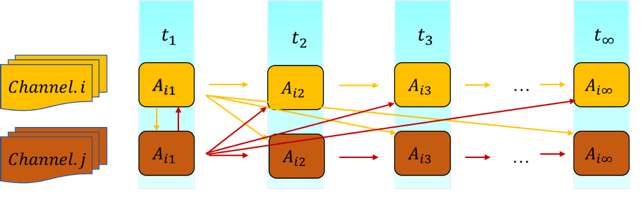
\includegraphics[width=0.8\textwidth]{2_ad_process}
% \caption{广告在两个渠道上的生命周期}
% \label{fig:2_ad_process}
% \end{figure}

% 对于本渠道自身延迟的效果影响,我们可以使用强化学习中的累积折扣奖赏最大化处理;而对其他渠道产生的影响,我们通常要对全部的渠道进行建模,以捕捉到渠道之间的联系,但是,在广告投放的场景中,我们所能获得的数据非常少,如果使用仅有的少量数据对全部渠道进行建模,那么得到的模型自然时很差的。所以,一个自然的想法是,我们应该对每个渠道进行单独的建模,然后通过启发式的经验改进值函数的评估方法。

% 假设含有$n$个渠道的集合为$I=\{1,2,\cdots,n\}$,在某时刻,其他渠道$I\backslash\{i\}$对渠道$i$产生的影响记为$q_{i}^{'}$,定义为:
% \begin{equation}\label{seq_ad_influence}
% \begin{aligned}
% q_{i}^{'}=\sum_{j\in I \backslash \{i\}} \sum_{k=0}^{\infty} \tau_{j,i,t+k+1} \cdot \gamma_{i}^{k} \cdot r_{j,t+k+1},\\
% \tau_{j,i,t+k+1}=d \cdot \frac{c_{j,t+k+1}}{c_{i,t+k+1}},d<1.
% \end{aligned}
% \end{equation}

% 式$\eqref{seq_ad_influence}$中,$\gamma_{i}$表示渠道$i$的折扣因子,$\tau_{j,i,t+k+1}$是一个常数$d$乘以$t+k+1$时刻在第$j$个渠道上的花费与在第$i$个渠道上花费之比,$r_{j,t+k+1}$表示渠道$j$在$t+k+1$时刻所获的即时利润。从公式中可以看出,$\sum_{k=0}^{\infty} \gamma_{i}^{k} \cdot r_{j,t+k+1}$是近似为其他某一渠道获得的所获的累积利润,$\tau_{j,i,t+k+1}$通过某时刻第$j$个渠道上的花费与第$i$个渠道上花费的比值来反映渠道$j$对渠道$i$的投放效果的影响。

% 于是,考虑$q_{i}^{'}$并结合公式\eqref{seq2_qsa},可以得到改进的渠道$i$最优值函数的公式:
% \begin{equation}
% \label{seq_modified_q}
% \begin{aligned}
% q_{i}(S_{t},A_{t})&=\mathbb{E}[\sum_{k=0}^{\infty} \gamma_{i}^{k} r_{i,r+k+1} + \sum_{j \in I \backslash \{i\}} \sum_{k=0}^{\infty} \tau_{j,i,t+k+1} \cdot \gamma_{i}^{k} r_{j,t+k+1} | S_{t}=s, A_t = a]\\
% &=\mathbb{E}[r_{i,t+1} + \gamma_{i} \sum_{k=0}^{\infty} \gamma_{i}^{k} r_{r+k+2} + \sum_{j \in \backslash \{i\}} \tau_{j,i,t+1}r_{j, t+1} \\
% &+ \gamma_{i} \sum_{j \in \backslash \{i\}} \sum_{k=0}^{\infty} \tau_{j,i,t+k+2} \cdot \gamma_{i}^{k} r_{j,t+k+2} | S_{t}=s, A_t = a]\\
% &=\mathbb{E}[r_{i,t+1} + \sum_{j \in I \backslash \{i\}} \tau_{j,i,t+1} r_{j, t+1} + \gamma_{i} q_{i}(S_{t+1},A_{t+1}) | S_{t}=s, A_t = a]\\
% \end{aligned}
% \end{equation}


% 因此,我们就可以将$t$时刻渠道$i$的Q值迭代的更新公式改为:
% % \begin{equation}
% % \begin{aligned}
% \begin{dmath}
% \label{seq_modified_Q}
% Q_{i}(S_{t},A_{t})=Q_{i}(S_{t},A_{t})+\alpha_{i}(r_{i, t+1} + \sum_{j \in I \backslash \{i\}} \tau_{j,i,t+1} r_{j, t+1} + \gamma_{i} max_{a_{'}} Q_{i}(S_{t+1}, a^{'}) - Q_{i}(S_{t},A_{t}))
% % \end{aligned}
% % \end{equation}
% \end{dmath}

% \subsection{改进的探索方法}
% 在传统的Q-learning学习方法中,我们通常采用的ε-greedy的探索方法。其思想为:以概率$\epsilon$随机选择一个行为,以(1-$\epsilon$)的概率选择最优的策略。 $\epsilon-greedy$平衡了利用(exploitation)和探索(exploration),其中选取动作值函数最大的部分为利用,其他非最优动作仍有概率为探索部分。但是这种方法存在两个弱点:第一,它只关心从行为中得到了多少奖赏,而不知道它对该行为了解多少,即所有行为在任何时候都是平等的。所以,即使某一行为在初试经历中没有获得奖赏,它仍然有会被探索到。第二,因为采用随机抽样的方法,所以很容易被负面的经历所干扰。因此,特别是在小数据集的情况下,$\epsilon-greedy$的探索方法是不完全适用于广告投放的场景中。所以,我们在探索中,我们要不仅考虑到我们对该行为的了解程度,而且要减少随机采样的操作。所以,我们可以使用如下方式来选择行为:
% \begin{equation}
% \begin{aligned}
% \argmax_{a}[Q(s,a)+\varphi \sqrt{\frac{ln n^{'}}{n_{a}^{'}}}]
% \end{aligned}
% \end{equation}
% 其中,$n^{'}$表示所有行为被选择的次数,$n_{a}^{'}$表示行为$a$被选择的次数,常数$\varphi > 0$控制了探索的程度。

% 因此,$t$时刻渠道$i$的Q值迭代的更新公式改为:

% \begin{dmath}
% \label{seq_modified_Q_}
% Q_{i}(S_{t},A_{t})=Q_{i}(S_{t},A_{t})+\alpha_{i}(r_{i, t+1} + \sum_{j \in I \backslash \{i\}} \tau_{j,i,t+1} r_{j, t+1} + \gamma_{i} \max_{a_{'}} Q_{i}(S_{t+1}, \argmax_{a^{'}}[Q(S_{t},A_{t})+ \varphi_{i} \sqrt{\frac{ln n_{i}^{'}}{n^{'}_{i a^{'}}}}]) - Q_{i}(S_{t},A_{t}))
% \end{dmath}



% \subsection{批处理以及整体架构}
% 经过上述改进Q值函数的迭代公式以及探索方法后,对SVR+Q+MCKP分块模型的流程也要做相应的改进。因为在更新Q值函数时,需要考到到其他渠道的影响,这就要求我们应该利用同一时刻的投放数据同时对所有渠道进行更新。同时,为了使训练过程更加符合真是的投放场景,参考文献\citep{pednault2002sequential}采取了批强化学习的训练方法。改进后的模型伪代码如算法\eqref{algo:RBF-SVR+Q_final}和算法\eqref{algo:RBF-SVR+Q_2}所示。

% \begin{algorithm}[htbp]
% \small
% \SetAlgoLined
% \SetKwRepeat{Repeat}{repeat}{until} 
% \SetKwData{Left}{left}\SetKwData{This}{this}\SetKwData{Up}{up}

% 输入:全部渠道的集合$I=\{1,2,\cdots,n\}$,$n$为渠道的总数;全部渠道的投放数据$O=\{O_{1},O_{2},\cdots,O_{n}\}$,其中$O_{i}=\{<\bm{s}_{i,t},c_{i,t},r_{i,t+1},\bm{s}_{i,t+1}>|t=1,\cdots,N_{i}\}$表示第$i$个渠道的数据集,$N_{i}$表示第$i$个渠道的数据量;Q函数的学习率$\alpha_{i}$,折扣因子$\gamma_{i}$,$i=1,2,\cdots,n$,最大迭代次数$P$,SVR+Q模型中的正则化参数$C$,RBF核函数的宽度$\sigma$\;

% \For{$i=1$ \KwTo $n$}{
% 	利用算法$\ref{algo:DC}$求出渠道$i$的离散区间$\bm{\omega}_{i}=\{\omega_{i,1},\omega_{i,2},\cdots,\omega_{i,M_{i}+1}\}$,$M_{i}$表示第$i$个渠道形成的离散区间的个数\;
% 	将每个区间样本的平均花费值作为该区间所对应的行为值$a$,并且将此行为值添加到该区间的每个样本中,样本格式变为:$<\bm{s}_{i,t},c_{i,t},a_{i,t},r_{i,t+1},\bm{s}_{i,t+1}>$ \;
% 	按照行为值的不同,建立为$M_{i}$个样本单元$D_{i,h}$,$h=\{1,\cdots,M_{i}\}$,且此时,$D_{i,h}=\varnothing$ \;
% }

% 数据转换:将全部渠道的数据$O$划分成$K$个情节$e$,即:$O=\{e_{k}|k=1,\cdots,K\}$,每个情节$e_{k}$包括$l_{k}$天的投放数据,即:$e_{k}=\{O^{'}_{j}|j=1,\cdots,l_{k}\}$,每一天的投放数据$O^{'}_{j}$又由$n$个渠道组成,即:$O^{'}_{j}=\{<\bm{s}_{k,j,i},c_{k,j,i},a_{k,j,i},r_{k,j+1,i},\bm{s}_{k,j+1,i}>|i=1,\cdots,n\}$\;

% % 新增输入数据:SVR+Q模型中的正则化参数$C_{i,j}$,RBF核函数的宽度$\sigma_{i,j}$,,其中$i=1,2,\cdots,n$表示渠道号,$j=1,2,\cdots,M_{i}$表示渠道所对应的离散行为个数\;

% \For{$k = 1$ \KwTo $K$}{
% 	\For{$j = 1$ \KwTo $l_{k}$}{
% 		\For{$i = 1$ \KwTo $n$}{
% 			按照算法\eqref{algo:RBF-SVR+Q_2}第10行的公式,计算样本的Q值,并将Q值添加到该样本中,其格式变为:$<\bm{s}_{k,j,i},c_{k,j,i},a_{k,j,i},r_{k,j+1,i},Q^{(0)}_{k,j,i}(\bm{s}_{k,j,i}),\bm{s}_{k,j+1,i}>$\;
% 			将该样本按照行为值分流到对应的样本单元中$D_{i,h}$,$h=\{1,\cdots,M_{i}\}$\;
% 		}
% 	}
% }
% $p=0$\;
% \Repeat{$p=P$}{
% 	SVR+Q分块多路逼近迭代过程(算法$\ref{algo:RBF-SVR+Q_2}$)\;
% 	$p=p+1$ \;
% }
% 输出各渠道的最终的Q值函数:$\text{Q}_{i}^{(P)}=\cup_{j=1,\cdots,l_{i}}\text{Q}_{i,j}^{(P)}$\; 
% 全渠道的Q值函数:$\text{Q}={\text{Q}_{i}^{(P)}}$,$i=1,\cdots,n$\;
% $Res = MCKP(B,\text{Q})$\;
% 输出:最终的分配策略$Res$\;
% \caption{SVR+Q+MCKP算法}
% \label{algo:RBF-SVR+Q_final}
% \end{algorithm}

% \begin{algorithm}[htbp]
% \small
% \SetAlgoLined
% \SetKwRepeat{Repeat}{repeat}{until} 
% 	\For{$i=1$ \KwTo $n$}{
% 		\For{$j=1$ \KwTo $M_{i}$}{
% 			对每个样本单元$D_{i,j}$,利用SVR+Q分块逼近模型进行回归建模,得到当前轮的Q值函数分块模型:$\text{Q}_{i,j}^{p}=f_{i,j}^{(p)}(\bm{s})=\sum_{m=1}^{N_{i,j}}(\hat{\alpha}_{i,j,m}^{(p)}-\alpha_{i,j,m}^{(p)})k(\bm{s},\bm{s}_{i,j,m})+b_{i,j}^{(p)}$,$N_{i,j}$表示第$i$个渠道的第$j$个样本空间中样本的个数\;
% 		}
% 	}

% 	\For{$k = 1$ \KwTo $K$}{
% 		\For{$j = 1$ \KwTo $l_{k}$}{
% 			\For{$i=1$ \KwTo $n$}{
% 				更新Q值函数:\\
% 				$\text{Q}_{k,j+1,i}^{(p+1)} = \text{Q}_{k,j+1,i}^{(p)} + \alpha_{i}^{(p)} (r_{k,j+1,i}+\gamma_{i} \argmax_{a^{'}}[f_{i,ID(a_{i}^{'})}^{(p)}(\bm{s}_{k,j+1,i})+\varphi_{i} \sqrt{\frac{ln n_{i}^{'}}{n_{i,ID(a_{i}^{'})}^{'}}}]) - \text{Q}_{k,j+1,i}^{(p)}$\;
% 				$ID(a_{i}^{'})$第$i$个渠道行为$a_{i}^{'}$所对应的编号,$n_{i}^{'}$ 为第$i$个渠道所有行为已经选择的次数,$n_{i,ID(a_{i}^{'})}^{'}$表示行为$ID(a_{i}^{'})$被选择的次数\;
% 				}
% 				利用上式更新在样本单元中的Q值\;
% 			}
% 		}

% \caption{SVR+Q分块逼近的迭代过程}
% \label{algo:RBF-SVR+Q_2}
% \end{algorithm}


\section{本章小结}
在本章中,首先分析了在直复营销体系下,基于广告代理商的投放预算分配问题,并说明了将全渠道的LTV作为评价广告投放效果的指标,以此作为选择强化学习解决该问题的出发点。另外,又分析在应用时所面临的场景复杂、数据量少以及预算约束等问题。然后,在小数据集下,针对值函数逼近问题提出了SVR+Q多路逼近模型,加快收敛速度的同时提高手链精度,并将SVR+Q与MCKP结合,应用于多渠道资金分配问题。最后,提出一个花费空间离散化的方法,以更好的应用SVR+Q+MCKP模型、针对多渠道之间的影响提出一种改进值函数的估计方法,而且提出了一个在小数据集下高效的探索方法。


